\documentclass[12pt,handout]{beamer}

% For fast compiling
%\includeonlylecture{intro}

% -- PACKAGES -- 
\usepackage{pgf}
\usepackage{pgfplots}
\usepackage{tikz}
\usetikzlibrary{patterns}
\usepackage{amsmath,amssymb,amsopn}
\usepackage[latin1]{inputenc}
\usepackage[english]{babel}
\usepackage{booktabs,colortbl}
\usepackage{subfigure}
\usepackage{import}
%\usepackage{algorithm}
\usepackage{algorithm}
%\usepackage{algorithmic}
\usepackage[noend]{algpseudocode}

\usepackage{graphicx}
\usepackage{cleveref}
\graphicspath{{./img/}}
%\newtheorem{lemma}[theorem]{Lemma}




\usepackage{biblatex}
\addbibresource{ref.bib}
\addbibresource{jcc-bib.bib}
\addbibresource{msip-bib.bib}
\addbibresource{dfo-bib.bib}



%-- Beamer setup --%

% Colors
%\definecolor{wisconsin-gold}{rgb}{0.8,0.6,0}
\definecolor{lehigh-gold}{rgb}{1,0.9,0.1}
\definecolor{wisconsin-red}{rgb}{0.6,0,0}

\definecolor{french-blue}{rgb}{0,0.1254,0.62}
\definecolor{french-red}{rgb}{0.96,0.16,0.25}

\usecolortheme[named=wisconsin-red]{structure}
\usetheme{Copenhagen}
\setbeamercolor{alerted text}{fg=wisconsin-red}

\usefonttheme[onlymath]{serif}
\useoutertheme{infolines}

\definecolor{illini-blue}{rgb}{0,0.247,0.58}
\definecolor{illini-orange}{rgb}{0.89,0.41,0.14}


\tikzset{
        hatch distance/.store in=\hatchdistance,
        hatch distance=10pt,
        hatch thickness/.store in=\hatchthickness,
        hatch thickness=2pt
    }

\makeatletter
    \pgfdeclarepatternformonly[\hatchdistance,\hatchthickness]{flexible hatch}
    {\pgfqpoint{0pt}{0pt}}
    {\pgfqpoint{\hatchdistance}{\hatchdistance}}
    {\pgfpoint{\hatchdistance-1pt}{\hatchdistance-1pt}}%
    {
        \pgfsetcolor{\tikz@pattern@color}
        \pgfsetlinewidth{\hatchthickness}
        \pgfpathmoveto{\pgfqpoint{0pt}{0pt}}
        \pgfpathlineto{\pgfqpoint{\hatchdistance}{\hatchdistance}}
        \pgfusepath{stroke}
    }


\makeatletter
    \pgfdeclarepatternformonly[\hatchdistance,\hatchthickness]{flexible hatch2}
    {\pgfqpoint{0pt}{0pt}}
    {\pgfqpoint{\hatchdistance}{\hatchdistance}}
    {\pgfpoint{\hatchdistance-1pt}{\hatchdistance-1pt}}%
    {
        \pgfsetcolor{orange}
        \pgfsetlinewidth{\hatchthickness}
        \pgfpathmoveto{\pgfqpoint{0pt}{0pt}}
        \pgfpathlineto{\pgfqpoint{\hatchdistance}{\hatchdistance}}
        \pgfusepath{stroke}
    }


\useframetitletemplate{%
\vskip0.25em%
\alert{\Large \insertframetitle}
\par
}

% -- Images you want to use more than once --

%\pgfdeclareimage[width=1cm]{wisconsin-logo}{images/wcrest} 
%\logo{\pgfuseimage{wisconsin-logo}}


%\pgfdeclareimage[width=0.1\textwidth]{flag-small}{images/Flag_of_France}


% -- Jeff's MACROS -- %

\newcommand{\picframetitle}[2]{
    \vskip0.25em%
    \begin{centering}
      \begin{minipage}[c]{0.7\linewidth}
	\Large \alert{#1}
      \end{minipage} \hfill
      \begin{minipage}[c]{0.22\linewidth}
	\pgfimage[height=0.5in]{#2}
      \end{minipage}
      \par
    \end{centering}
}

\newcommand{\medpicframetitle}[2]{
    \vskip0.25em%
    \begin{centering}
      \begin{minipage}[c]{0.7\linewidth}
	\Large \alert{#1}
      \end{minipage} \hfill
      \begin{minipage}[c]{0.22\linewidth}
	\pgfimage[height=0.75in]{#2}
      \end{minipage}
      \par
    \end{centering}
}

\newcommand{\bigpicframetitle}[2]{
    \vskip0.25em%
    \begin{centering}
      \begin{minipage}[c]{0.7\linewidth}
	\Large \alert{#1}
      \end{minipage} \hfill
      \begin{minipage}[c]{0.22\linewidth}
	\pgfimage[height=1in]{#2}
      \end{minipage}
      \par
    \end{centering}
}

\newcommand{\bigpicframetitletwo}[2]{
    \vskip0.25em%
      \begin{minipage}[c]{0.6\linewidth}
	\Large \alert{#1}
      \end{minipage} \hfill
      \begin{minipage}[c]{0.32\linewidth}
	\hfill \pgfimage[height=0.8in]{#2}
      \end{minipage}
      \par
}

\newcommand{\bigpicframetitlethree}[2]{
    \vskip0.25em%
      \begin{minipage}[c]{0.6\linewidth}
	\Large \alert{#1}
      \end{minipage} \hfill
      \begin{minipage}[c]{0.32\linewidth}
	\hfill \pgfimage[height=0.8in]{#2}
      \end{minipage}
      \par
}

\newcommand{\bi}{\begin{itemize}}
\newcommand{\ei}{\end{itemize}}
\newcommand{\BI}{\begin{itemize}}
\newcommand{\EI}{\end{itemize}}
\newcommand{\BEN}{\begin{enumerate}}
\newcommand{\EEN}{\end{enumerate}}

\newcommand{\BBR}[1]{\begin{beamerboxesrounded}[shadow=true,width=0.96\textwidth]{\color{lehigh-gold}#1}}
\newcommand{\EBR}{\end{beamerboxesrounded}}

\newcommand{\BCS}{\begin{columns}}
\newcommand{\BC}[1]{\begin{column}{#1\linewidth}}
\newcommand{\EC}{\end{column}}
\newcommand{\ECS}{\end{columns}}

\newcommand{\MSS}{\medskip\alert{\hrule}\medskip}
\newcommand{\BSS}{\bigskip\alert{\hrule}\bigskip}
\newcommand{\st}{\; | \;}

\newcommand{\noprint}[1]{}
\newcommand{\exclude}[1]{}
\newcommand{\cB}{{\cal B}}
\newcommand{\cC}{{\cal C}}
\newcommand{\cD}{{\cal D}}
\newcommand{\cE}{{\cal E}}
\newcommand{\cF}{{\cal F}}
\newcommand{\cG}{{\cal G}}
\newcommand{\cI}{{\cal I}}
\newcommand{\cK}{{\cal K}}
\newcommand{\cL}{{\cal L}}
\newcommand{\cN}{{\cal N}}
\newcommand{\cO}{{\cal O}}
\newcommand{\cP}{{\cal P}}
\newcommand{\cQ}{{\cal Q}}
\newcommand{\cR}{{\cal R}}
\newcommand{\cS}{{\cal S}}
\newcommand{\cT}{{\cal T}}
\newcommand{\cU}{{\cal U}}
\newcommand{\cX}{{\cal X}}
\newcommand{\cV}{{\cal V}}
\newcommand{\cZ}{{\cal Z}}

\newcommand{\magE}{\left| \mathcal{E} \right|}

\newcommand{\defeq}{\stackrel{\rm def}{=}}
\newcommand{\Expect}{\mathbb{E}}

\newcommand{\orb}{\operatorname{orb}}


\newcommand{\ry}{\pmb{y}}
\newcommand{\rye}{\pmb{y_e}}

\makeatletter
\def\BState{\State\hskip-\ALG@thistlm}
\makeatother

\newcommand{\mypathjcc}{../thesis/jcc}
\newcommand{\mypathjccdata}{../thesis/jcc/data}
\newcommand{\bE}{\mathbb{E}}
\newcommand{\E}[2]{\mathbb{E}_{#1} \left[ #2 \right]}
\newcommand{\bP}[2]{\mathbb{P}_{#1} \left[ #2 \right]}
\newcommand{\dpO}{d\mathbb{P}_\Omega}
\newcommand{\feb}{f_e\left(\beta\right)}
\newcommand{\fenb}{f_{en}\left(\beta\right)}
\newcommand{\fehb}{f_e\left(\hat{\beta}\right)}
\newcommand{\pfeb}{\frac{\partial}{\partial \beta_j}\feb}
\newcommand{\pfenb}{\frac{\partial f_{en}\left(\beta \right)}{\partial \beta_j}}
\newcommand{\pfehb}{\frac{\partial f_e\left(\hat{\beta} \right)}{\partial \beta_j}}
\newcommand{\hye}{\hat{y}_e}
\newcommand{\hse}{\hat{s}_e}
\newcommand{\pe}{\pi_e}
\newcommand{\pn}{\pi_n}
\newcommand{\psen}{\psi_{en}}
\newcommand{\rand}{\boldsymbol{\delta}}
\newcommand{\ri}{\pmb{\delta^m}}
\newcommand{\rf}{\pmb{\delta^y}}
\newcommand{\rx}{\pmb{x}}
\newcommand{\rD}{\pmb{\Delta}}
\newcommand{\rdm}{\pmb{\delta^m}}
\newcommand{\rdmk}{\pmb{\delta^m_k}}
\newcommand{\rdy}{\pmb{\delta^y}}
\newcommand{\hry}{\pmb{y}}
\newcommand{\hy}{y}
\newcommand{\rz}{\pmb{z}}
\newcommand{\sD}{\sigma_\Delta^2}
\newcommand{\se}{\sigma_e^2}
\newcommand{\sn}{\sigma_n^2}
\newcommand{\sen}{\sigma_{en}^2}
\newcommand{\see}{\sigma_{ee}^2}
\newcommand{\sko}{\sum_{k_1}}
\newcommand{\skt}{\sum_{k_2}}
\newcommand{\sigot}{\Sigma_{k_1,k_2}}
\newcommand{\irzp}{\E{\Omega}{g(\hry_e)}}
%\newcommand{\rw}{{w(\omega)}} %\newcommand{\rx}{{x(\omega)}} %\newcommand{\ry}{{y(\omega)}}
\newcommand{\Ery}{\E{\Omega}{\ry}}
\newcommand{\Erx}{\E{\Omega}{\rx}}
\newcommand{\Erdm}{\E{\Omega}{\rdm}}
\newcommand{\ErD}{\E{\Omega}{\rD}}
\newcommand{\tB}{\tilde{B}}
\newcommand{\tx}{\tilde{x}}
\newcommand{\ttheta}{\tilde{\theta}}

\title[Cascading Power Failures]{Computational Models for Risk and Reliability on~Bulk~Power~Systems}
\author{Eric Anderson}
\institute{UW Madison}
\date{December 10th, 2014}

\begin{document}

\begin{frame}
\titlepage
\end{frame}



\subsubsection{Outline}
\frame{Outline \hfill Percent Complete

\tableofcontents[subsubsectionstyle=hide]  }


\section{Modeling Cascading Power Failures, Ch. 2 \hfill (92\%)}
\frame{\tableofcontents[currentsection,subsubsectionstyle=hide]}
\subsection{Cascading Power Failures}
\begin{frame}{Modeling Cascading Power Failures}
\textbf{Cascading power failure} is a process in which an outage on the power grid weakens the system and shifts load, which in turn causes another outage, and so forth

\alert{Outline}
\begin{itemize}
\item The Real World Problem
\item Model of Cascading Power Failures
%\bi
%\item Equillibrium and Critical Points
%\ei
\item Multi-stage stochastic program
%\bi
%\item Effective capacity and a priori sampling
%\item Decision dependent uncertainty
%\item Binary variables for line failures
%\ei
\item Planning Models (Transmission Expansion)

\end{itemize}
\end{frame}

\subsubsection{Reliability Problems}
\begin{frame}{Reliability Problems}
\alert{Cascading power failures}
\bi
\item Rare, but costly
\item Power tail distribution, unchanged for 30 years
\item Northeast blackout 2003
\bi
\item \$6 billion economic loss
\item Loss of life
\ei
\ei
\pause
\alert{Power Interruptions}
\bi
\item \$79 billion economic loss (2001) 
\bi
\item \$247 billion electricity sales
\ei 
\item Hidden from system, distributed throughout economy
\item New technologies: renewables, EVs, etc. stressful on system
\ei
\end{frame}


\subsubsection{OPA Model}
\begin{frame}{Forces on System}
Full OPA (Oak Ridge, PSERC Wisc., and Alaska) model tries to capture these forces and find an equillibrium that is seen in the real world \newline \\
\pause
Short Term Forces:
\begin{itemize}
\item Random demand fluctuations
\item \alert{Blackouts, Cascading Process}
\item Dispatch Model
\end{itemize}
\pause
Long Term Forces:
\begin{itemize}
\item Economic and political processes
\item System repair
\item Load growth
\item Design and upgrade of system
\end{itemize}
\end{frame}


\subsubsection{Dynamic Equilibrium}
\begin{frame}{Equilibrium}
Self-organized into dynamic equilibrium where blackouts of all sizes occur\newline
\\ 
\pause
Average frequency of blackouts steady for 30 years
\bi
\item Changes seasonally and with time of day
\item Power tail distribution, exponent around $-1.3\pm.2$
\ei
\vspace{10pt}
\pause

\textbf{Critical Points} maximum system throughput
\bi
\item Limited by transmission constraints, large blackout, less  frequent
\item Limited by generation capacity, smaller blackout, more frequent 
\ei

\end{frame}

\subsubsection{OPA Simulation}
\begin{frame}{Cascade Simulation }
Hard to predict how cascade propagates, this rough cut simulation mimics distribution of real power outages, a heavy tailed distribution \newline  \\
\begin{center}
\begin{tikzpicture}[scale=1.3]
\draw [->,thick] (1,1) node[anchor=east,label=below:occurs]{$\xi$}
-- (1.35,1) node(TC)[anchor=west,text width=1.4cm,text centered,  rectangle, draw]{\scriptsize Topology Changes};
\draw[->,thick] (TC)
--(3.1,1) node(PF)[anchor=west,text width=1.4cm,text centered, rectangle,draw]{\scriptsize Power Flow Calculated};
\draw[->,thick] (PF)
--(5,1) node(F)[anchor=west,text width=1.5cm, text centered, rectangle, draw]{\scriptsize Overloaded Lines Fail, Probability $p$};
\draw[->,thick] (F)
--(7.2,1) node(DN)[anchor=west,text width=1.5cm, text centered,rectangle,draw]{\scriptsize No Failures, Cascade Done};
\draw[->,thick] (F.south west)
--(4.6,-.5) node(LF)[anchor=east,text width=1.6cm, text centered, rectangle, draw]{\scriptsize Line Failures };
\draw[->,thick] (LF.west)
-- (TC.south east);

\end{tikzpicture} 
\end{center}

%Initial event $\xi$ happens \newline  
%Power Flow calulated for new system \newline 
%If a line is at its limit, it will fail with a given probability\newline  
%Once the new set of outages is found, the process repeats by calculating new power flow
\end{frame}



\frame{
\frametitle{Visualizing a Cascade}

\BCS
\BC{0.7}
\centering
\begin{tikzpicture}[line width=2pt]

\node[circle,fill=red!20] (one) at (3,0) {1};
\node[circle,fill=red!20] (two) at (5,0) {2};
\node[rectangle,fill=green!20] (three) at (7,1) {3};
\node[rectangle,fill=green!20] (four) at (5,1.75) {4};
\node[rectangle,fill=green!20] (five) at (3,1.75) {5};
\node[circle,fill=red!20] (six) at (2,3) {6};
\node[rectangle,fill=green!20] (seven) at (5,3) {7};
\node[circle,fill=blue!20] (eight) at (4,3.5) {8};
\node[rectangle,fill=green!20] (nine) at (7,3) {9};
\node[rectangle,fill=green!20] (ten) at (6,4) {10};
\node[rectangle,fill=green!20] (eleven) at (3,5) {11};
\node[rectangle,fill=green!20] (twelve) at (2,5) {12};
\node[rectangle,fill=green!20] (thirteen) at (1,4) {13};
\node[rectangle,fill=green!20] (fourteen) at (4,6) {14};

\invisible<2->{\draw[red] (one) -- (two) ;}
\invisible<2->{\draw (one) -- (five);}
\invisible<3->{\draw<2->[red] (one) -- (five) ; }
\invisible<2->{\draw[red] (two) -- (three) ; }
\invisible<2->{\draw[red] (two) -- (four) ; }
\draw (two) -- (five) ; 
\invisible<2->{\draw[red] (three) -- (four) ; }
%\invisible<2->{\draw[red] (four) -- (five) ; }
\draw (four) -- (five) ; 
\invisible<4->{\draw (four) -- (seven);}
\invisible<5->{\draw<4->[red] (four) -- (seven) ;}
\invisible<4->{\draw (four) -- (nine);}
\invisible<4->{\draw<3->[red] (four) -- (nine) ; }
\draw (five) -- (six) ; 
\invisible<2->{\draw[red] (six) -- (eleven) ; }
\draw (six) -- (twelve) ; 
\draw (six) -- (thirteen) ; 
\draw (seven) -- (eight) ; 
\invisible<2->{\draw[red] (seven) -- (nine) ; }
\draw (nine) -- (ten) ; 
\draw (nine) .. controls +(up:1.2cm) .. (fourteen) ; 
\draw (ten) -- (eleven);
%\invisible<5-> {\draw<4->[red] (ten) -- (eleven) ;  }
\invisible<3->{\draw (twelve) -- (thirteen);}
\invisible<5-> { \draw<3- >[red](twelve) -- (thirteen) ; }
\draw (thirteen) .. controls +(up:1.2cm) .. (fourteen) ; 
\end{tikzpicture}
\EC
\BC{0.3}
\BI
\item<2->{Original Fault}
\item<3->{$t=2$, Line $(1,5)$ fails}
\item<4->{$t=3$, Line $(4,7)$ fails}
\item<5->{$t=4$, \alert{Few Lines Out}}
\item<6->{No lines overloaded, cascade done}
\EI
\EC
\ECS

}

\begin{frame}{Cascade Review}
At each stage, OPA minimizes load shed first and foremost!
\pause
\bi
\item \alert{OPA is GREEDY!}
\item Need to capture this behavior
\bi
\item Load shed early to avoid large blackouts
\item Then distribution does not match
\ei
\ei
\begin{center}
\begin{tikzpicture}[scale=1.3]
\draw [->,thick] (1,1) node[anchor=east,label=below:occurs]{$\xi$}
-- (1.35,1) node(TC)[anchor=west,text width=1.4cm,text centered,  rectangle, draw]{\scriptsize Topology Changes};
\draw[->,thick] (TC)
--(3.1,1) node(PF)[anchor=west,text width=1.4cm,text centered, rectangle,draw]{\scriptsize \alert{Power Flow Calculated}};
\draw[->,thick] (PF)
--(5,1) node(F)[anchor=west,text width=1.5cm, text centered, rectangle, draw]{\scriptsize Overloaded Lines Fail, Probability $p$};
\draw[->,thick] (F)
--(7.2,1) node(DN)[anchor=west,text width=1.5cm, text centered,rectangle,draw]{\scriptsize No Failures, Cascade Done};
\draw[->,thick] (F.south west)
--(4.6,-.5) node(LF)[anchor=east,text width=1.6cm, text centered, rectangle, draw]{\scriptsize Line Failures };
\draw[->,thick] (LF.west)
-- (TC.south east);

\end{tikzpicture} 
\end{center}



%Initial event $\xi$ happens \newline  
%Power Flow calulated for new system \newline 
%If a line is at its limit, it will fail with a given probability\newline  
%Once the new set of outages is found, the process repeats by calculating new power flow
\end{frame}



\subsection{Multi-Stage Stochastic Program}
\begin{frame}{Super Model}
\BBR{Multi-Stage Stochastic Program (IP-OPA)}
\begin{itemize}
\item Mathematical model of OPA
\item Gives flexibility to use as sub-model in design problems
\item Computationally difficult
\begin{itemize}
\item Decision dependent uncertainty
\bi
\item Model with binary variables
\item Sampling done a priori
\ei
\item Large sample size makes IP-OPA difficult
\end{itemize}
\end{itemize}
\EBR
\end{frame}
\begin{frame}{Scenario Tree}
The OPA simulation will be built using a scenario tree
\bi
\item Cascade evolves depending on decision at $n$
\bi
\item Each node has DC power flow
\ei
\item Branch factor $M$ determines resolution of uncertainty
\ei
\begin{center}
\begin{tikzpicture}[scale=.80]

\draw (-1,2.5) node(RHO)[circle,draw,scale=.8]{\small $\rho(n)$ };
\draw (2,2.25) node(NUP)[circle,dashed,scale=2.4,draw]{ };
\draw (2,1) node(N)[circle,scale=1.5,draw]{\scriptsize $n$ };
\draw (2,-.25) node(NDOWN)[circle,dashed,scale=2.4,draw]{ };
\draw (5,2.5) node(N1)[circle,scale=1,draw]{\scriptsize $n_1$ };
\draw (5,1.5) node(N2)[circle,scale=1,draw]{\scriptsize $n_2$ };
\draw (5,-.5) node(NO)[circle,scale=1,draw]{\scriptsize $n_M$ };

\draw[thick,dashed, ->] (RHO) -- (NUP);
\draw[thick,->] (RHO) -- (N);
\draw[thick,dashed, ->] (RHO) -- (NDOWN);
\draw[thick,->] (N) -- (N1);
\draw[thick,->] (N) -- (N2);
\draw[thick,->] (N) -- (NO);
\draw[thick,dashed] (N2) -- (NO);

\draw[thick] (-2,-1.5) -- (5.5,-1.5);
\draw[thick] (-1, -1.75) -- (-1, -1.25);
\draw[thick] (2, -1.75) -- (2, -1.25);
\draw[thick] (5, -1.75) -- (5, -1.25);

\draw(-2.2,-2) node {Stage};
\draw(-1,-2) node {$t-1$};
\draw(2,-2) node {$t$};
\draw(5,-2) node {$t+1$};

\end{tikzpicture} 
\end{center}
\end{frame}


\begin{frame}{DC Power Flow}
Lossless power flow and nominal voltage magnitudes.
\begin{align*}	\displaystyle
\sum_{j \in \cV}{f_{ijn}} &= p_{in} -d_{in} \hspace{20px}   \forall i \in \cV, \forall n \in \cN   
\\
\theta_{in} - \theta_{jn} &= X_{ij} f_{ijn}			\hspace{20px}	\forall i,j \in \cV, \forall n \in \cN   
\end{align*}

\begin{itemize}
\item Linear
%\begin{itemize}
%\item Can use MIP, not MINLP
%\end{itemize}
\item Common approximation used in most economic models
\end{itemize}
\end{frame}

%\subsection{Decision Dependent Uncertainty}
\begin{frame}{Probablistic Branch Failure}
Model branch failures dependent on current flow
\pgfplotsset{every axis plot/.append style={line width=2pt}}
\tikzset{
every pin/.style={fill=yellow!50!white,rectangle,rounded corners=3pt,font=\tiny},
small dot/.style={fill=black,circle,scale=0.3}
}
\begin{center}
\begin{tabular}{c c}
\begin{tikzpicture}[scale=.65]
\begin{axis}[ 
	xlabel=$f$,
	ylabel=$P( R < f )$,
	title = OPA Simulation Failure PDF,
	unbounded coords = jump,
	xtick= {0},
	ytick= {0, 1},
	extra y ticks={.5},
	extra y tick style={grid=major},
	extra y tick labels={$p$},
	extra x ticks={.575,1},
	extra x tick labels={$L$, $U$},
        ymax=1.1,
        xmax=1.1,
scatter/classes={
 		 a={mark=o,line width=3.5pt},%
 		 b={mark=o,line width=1pt,scale=1.75}%
		}]
	\addplot[black] coordinates { 
		(0,0)		
		(.985,0)	
%		(,.485) 		
%		(1,inf)		
%               (1,1)		
		};	
	\addplot[ 
		scatter,only marks,
		scatter src=explicit symbolic]
		coordinates {  
		(0,0)		[a]
		(1,0)		[b]
		(1,.5)		[a]
		(1,1)		[b]

		};
	\addplot[black] coordinates { 
		(1.025,1)		
		(2,1)		
		};	

	

\end{axis}
\end{tikzpicture}
&
\begin{tikzpicture}[scale=.65]
\begin{axis}[ 
	xlabel=$f$,
	ylabel=$P( R < f )$,
	title = Effective Capacity PDF,
	unbounded coords = jump,
	xtick= {0},
	ytick= {0, 1},
	extra y ticks={.5},
	extra y tick style={grid=major},
	extra y tick labels={$p$},
	extra x ticks={.575,1},
	extra x tick labels={$L$, $U$},
        xmax=1.1,
scatter/classes={
 		 a={mark=o,line width=3.5pt},%
 		 b={mark=o,line width=1pt,scale=1.75}%
		}]
	\addplot[black] coordinates { 
		(0,0)		
		(.575,0)	
		(.985,.485) 		
		(1,inf)		
		(1,1)		
		};	
	\addplot[black] coordinates { 
		(1.025,1)		
		(2,1)		
		};	
	\addplot[ 
		scatter,only marks,
		scatter src=explicit symbolic]
		coordinates {  
		(0,0)		[a]
		(1,.5)		[a]
		(1,1)		[b]
		};


	

\end{axis}
\end{tikzpicture}
\end{tabular}
\end{center}
Effective capacity reduces ``cheating''
\end{frame}


\begin{frame}{Sampling}
Line Failure if $f_e \ge \alpha U_e$ and $w_{ne} =1$.  
\begin{itemize}
\item $\omega_n \equiv\left[ 0, 0, 1, 0, \cdots, 1\right]$	from Bernouillli with prob. $p$
\item $\alpha_n \equiv\left[ .75, .85, .52, .67, \cdots, .93\right]$	from Uniform $\left[ L_{ij}, U_{ij} \right]$
\end{itemize}

Effective capacity to incorporate this information.    
\begin{equation*}
 R_{ne} = 
 \left\{ 
	\begin{array}{lr}
				\alpha_{ne} U_e & \mbox{if } \omega_{ne}=1\\
			  U_e + \epsilon & \mbox{if } \omega_{ne}=0
	\end{array}
 \right. 
\end{equation*}
\pause
\BBR{Effective capacity in Big-M constraints to "switch'' outaged lines}
\begin{itemize}
\item The power flow on the given branch must be fixed to 0
\item The equation relating phase angles of two connected components removed
\end{itemize}
\EBR

\end{frame}



\begin{frame}{Decision Dependent Uncertainty}
Line fails if power flow is greater than effective capacity
\begin{align*}
\mbox{If }
		\hspace{30px}&\left| f_{e\rho(n)} \right| > R_{en}  \\
\mbox{Then }
		\hspace{30px}&z_{en} = 0
\end{align*}
\pause
To model this logic, a Big-M constraint can be used, where M represents a large number.
\begin{align*}
	f_{e\rho(n)} - R_{en} &\le M^R_e (1-z_{en})	\\
	f_{e\rho(n)} + R_{en} &\ge - M^R_e (1-z_{en})	
\end{align*}
with $M^R_e = U_e - R_e$. \\

\end{frame}

\begin{frame}{Decision Dependent Uncertainty}
When the line is unavailable, 
\begin{itemize}
\item Power flow on that branch is zero 
\item Phase angles between the two nodes are not constrained
\end{itemize}
\begin{align*}
\mbox{If }
		\hspace{20px}&z_{en} = 0	\\
\mbox{Then }
		\hspace{20px}&f_{en} = 0  \hspace{10px} \mbox{ and}\\
				&\theta_{in} - \theta_{jn} - X_{e}f_{en} \mbox{ is arbitrary}
\end{align*}	

\pause
This can be achieved through the following equations.
\begin{align*}
-U_{e} z_{en} \le f_{en} &\le U_{e} z_{en}	\\
\theta_{in} - \theta_{jn} + X_e f_{en} &\ge -M^\theta_e(1-z_{en}) \\
\theta_{in} - \theta_{jn} + X_e f_{en} &\le M^\theta_e(1-z_{en})  
\end{align*}
with $M^\theta_e = 2 \theta_{max} + X_e U_e$.

\end{frame}


\subsubsection{Cascade Submodel}

\begin{frame}{Cascade Submodel}
The cascading process begins
\begin{itemize}
\item Intial exogenous event, $\xi \in \left\{ 0, 1 \right\}^{\magE}$.  
\item Line outaged for all $\xi = 1$.
\end{itemize}
\begin{equation*}
z_{en} \le 1- \xi_e  
\end{equation*}
\pause
Feasible region for cascading given effective capacity sampling
\begin{equation*}
\cX (\alpha, \omega, \xi) \equiv \left\{ \left(d, p, f, z \right)  |  \mbox{ DC power flow, cascade constraints  hold} \right\} 
\end{equation*}

\pause
\BBR{Economic Dispatch with Cascading Subproblem (IP-OPA)}
\begin{align*} \displaystyle
	{\large \mbox{min}} \hspace{10px} &  \Expect_\Omega \sum_{in} \left[ C_{in}  p_{in,m}  + W_{in} (\hat{d}_{i} - d_{in,m}) \right]	\\
	&(d,p,f,z)_m  \in \cX (\alpha_m, \omega_m, \xi_m)    \hspace{20px}   \forall (\alpha_m,\omega_m,\xi_m) \in \Omega
\end{align*}
\EBR
\end{frame}

\begin{frame}{Load Shed Distribution Matches}
The IP-OPA formulation has similar load shed distribution

\begin{figure}
 \centering
	\begin{tikzpicture}
		\begin{axis}[xlabel=$LS$ (MW), ylabel=$P($Load Shed $> LS )$
				,legend pos=north east
				,grid=major,
				,xmin=-25,xmax=400
				,title=\mbox{Load Shed Distribution} ]


 	\addplot[black,line width=3pt] table[x=mv, y=mp] {./data/calibrate.txt};
	\addlegendentry{MSIP}
	
	\addplot[red,line width=2pt] table[x=sv, y=sp,mark=square] {./data/calibrate.txt};
	\addlegendentry{SIM}





		\end{axis}	
	\end{tikzpicture}
  \caption{Load Shed Distribution for the OPA simulation and MSIP formulation}
 \label{dist}
\end{figure}

\end{frame}



\subsection{Transmission Expansion}
\begin{frame}{Transmission Expansion}
Embed IP-OPA as subproblem
\pause
\begin{itemize}
\item $\xi \in \Xi$ identified as primary risk for initiating a cascading event
\item Budget to use for expansion
\item Allocate budget to minimize risk measure of load shed
\end{itemize}
\pause
Let $x$ be the design variable
\begin{itemize}
\item First stage variable
\item Additional capacity on power lines
\end{itemize}
\pause
Effective capacity is affected
\begin{align*}
-(U_{e}+x_e) z_{en} \le f_{en} \le (U_{e}+x_e) z_{en} &		\\
 R_{ne} = 
 \left\{ 
	\begin{array}{lr}
				\alpha_{ne} (U_e + x_e) & \mbox{if } \omega_{ne}=1\\
			  (U_e + x_e) + \epsilon & \mbox{if } \omega_{ne}=0
	\end{array}
 \right. 
\end{align*}
\end{frame}


\begin{frame}{Scenario Tree}
\centering
\begin{equation*}
\cX (x, \alpha, \omega, \xi) \equiv \left\{ \left(d, p, f, z \right)  |  \mbox{ DC, cascade, effective capacity} \right\} 
\end{equation*}

\begin{tikzpicture}[scale=1]

\draw (.5,.5) node(ROOT)[circle,draw]{\small $x$ };
\draw (3,3) node(ONE)[circle,draw]{ \small $\cX_1$ };
\draw (3.25,1.5) node(TWO)[circle,draw]{ \small $\cX_2$ };
\draw (3.25,.85) node(DOTONE){ \large $\vdots$ };
\draw (3.25,0) node(N)[circle,dashed,draw]{ \small $\cX$ };
\draw (3.15,-.65) node(DOTTWO)[rotate=-15]{ \large $\vdots$ };
\draw (3,-1.5) node(S)[circle,draw]{ \small $\cX_M$ };

\draw (1.85,2.15) node(OMG1){ \small $\xi_1$ };
\draw (2.05,1.25) node(OMG2){ \small $\xi_2$ };
\draw (2.1,.4) node(OMG){ \small $\xi$ };
\draw (1.9,-.35) node(OMGS){ \small $\xi_M$ };

\draw[thick, ->] (ROOT) -- (ONE) ;
\draw[thick,->] (ROOT) -- (TWO);
\draw[thick,dashed, ->] (ROOT) -- (N);
\draw[thick,->] (ROOT) -- (S);

%\draw[thick,dashed] (TWO) -- (N);
%\draw[thick,dashed] (N) -- (S);

\end{tikzpicture} 

\end{frame}

\begin{frame}{Transmission Expansion}
\BBR{Budget}
\begin{itemize}
\item $\underline{B}_e,\overline{B}_e$ minimum,maximum capacity for each line
\item $B_x$ total capacity to add
\item $B_y$ total lines to change
\end{itemize}
\EBR
\begin{subequations}
\begin{align*} \displaystyle
	{\large \mbox{min}} \hspace{10px} &  \Expect_\Xi \sum_{in} \left[ C_{in}  p_{in,m}  + W_{in} (\hat{d}_{i} - d_{in,m}) \right]	\\
	&(d,p,f,z)_m  \in \cX(x,\alpha_m,\omega_m,\xi_m)    \hspace{20px}   \forall (\alpha_m,\omega_m,\xi_m) \in \Omega	\\
	& \underline{B}_e y_e \le x_e \le \overline{B}_e y_e \hspace{35px} \forall e \in \cE\\
	&\sum_e x_e \le B_x 	\\
	& \sum_e y_e \le B_y  
\end{align*}
\end{subequations}
\end{frame}
\begin{frame}{Computationally Difficult}
To hope to solve
\bi
\item Initial contingencies $\approx 4$
\item Stages $\approx 4$
\item Branching $\approx 3$
\ei

Sometimes solve
\bi
\item Sometimes 40-100\% optimality gap
\ei
\end{frame}
\begin{frame}{Results}
This is an example of a good result
\begin{center}
	\begin{tikzpicture}[scale=.6]
		\begin{axis}[xlabel=$LS$ (MW), ylabel=$P($Load Shed $> LS )$
				,legend pos=north east
				,grid=major,
				,xmin=-25,xmax=1300
				,title=\mbox{Load Shed Distribution} ]


 	\addplot[red,line width=2pt] table[x=ls, y=prob] {./data/d25k20.dat};
	\addlegendentry{design}
	
	\addplot[blue,line width=2pt] table[x=ls, y=prob,mark=square] {./data/dumb25k20.dat};
	\addlegendentry{heuristic}

	\addplot[black,line width=2pt] table[x=ls, y=prob,mark=square] {./data/sim.dat};
	\addlegendentry{nom}

		\end{axis}	
	\end{tikzpicture}
\end{center}
\vspace{-15pt}
\bi
\item But not all good!
\item Many performed similar to heuristic
\item Averaging many solves helped
\bi
\item Can't represent enough uncertainty
\ei
\ei
\end{frame}

\section{Risk Model for Real-Time Dispatch, Ch. 4 \hfill (78\%)}
\frame{\tableofcontents[currentsection,subsubsectionstyle=hide]}
\begin{frame}{Risk Model for Real-Time Dispatch}
Previous model for long term design problems
\bi
\item Solve in last section
\ei

What to do in real time to reduce line loading risk?
\pause

\alert{Outline}
\bi
\item Traditional DC dispatch
\item Analysis under net injection uncertainty
\item Line failure density function and system risk
\item JCC model and cost-risk frontier
\ei

\end{frame}

\subsection{DC Dispatch and Uncertainty}
\begin{frame}{DC Power Flow}
DC Power Flow equations  \alert{(notation change)}
\pause
\begin{align*}
y&=B' C \theta \\
x &= C^T y \\
x & = B \theta
\end{align*}
\pause
\begin{tabular}{c l}
$x$ & Net injections, $x<0 \equiv $demand (N)\\
$y$ & Branch flows (E)\\
$\theta$ & Phase angle (N)\\
$B'$ & Diagonal branch susceptance matrix (E x E)\\
$B$ & System matrix (N x N)\\
$C$ & Node-arc incidence matrix (E x N)\\
\end{tabular}

\pause
N-Number of nodes, E-Number of edges 


\end{frame}


\begin{frame}{DC Optimal Power Flow}
Economic dispatch with quadratic cost function
\begin{alignat*}{3}
\min_{\left(x;\theta,y\right)} && \displaystyle\sum_j \left[  c_2 x_j^2 + c_1 x_j \right.&\left.+ c_0 \right] &   \\
                        && \textstyle \sum_j C^g_{ij} x_j - \sum_e C^b_{ie} y_e          &=d_i       && \forall i \\ 
                 && y_e - b_e \textstyle \sum_i C^b_{ie} \theta_i          &=0         && \forall e \\
                 && y_e &\in \left[ -U_e, U_e \right] && \forall e\\
                 && x_j &\in \left[ G^{min}_j, G^{max}_j \right] && \forall j  
\end{alignat*}
\end{frame}

\subsubsection{Gaussian Flow and Risk Function}

\begin{frame}{Gaussian Injects}
\alert{Net Injection Uncertainties}
\bi
\item Subset of nodes have uncertain injections (i.e. wind)
\item Model as Gaussian
\ei
\pause
\begin{equation*}
 \rx = C_g\left(\alert{x_g}+\rD\alert{\beta}\right) - (d + C_M \ri) 
\end{equation*}

\pause
\begin{tabular}{ c l}
$\rx$ & Net injects \\
$x_g$ & Generator dispatch \\
$\beta$ & Slack distribution \\
$d$ & Expected demand \\
$\ri$ & Nodal demand variation ($\mathbb{E} \left[ \ri \right] = 0$, $\Sigma$ known)\\
$\rD$ & Aggregate demand variation ($\rD = 1^T \rdm$)
\end{tabular}

\end{frame}


\begin{frame}{DC OPF with Arbitrary Slack}
Take expectation of all terms
\pause
\bi
\item Only quadratic term is different
\ei
\begin{alignat*}{3}
\min_{\left(x,\beta;\theta,y\right)} && \displaystyle\sum_j \left[  c_2 \left(x_j^2 + \beta_j^2 \sD \right) \right. &\left.+ c_1 x_j + c_0 \right] &   \\
                        && \textstyle \sum_j C^g_{ij} x_j - \sum_e C^b_{ie} y_e          &=d_i       && \forall i \\ 
                 && y_e - b_e \textstyle \sum_i C^b_{ie} \theta_i          &=0         && \forall e \\
                 && y_e &\in \left[ -U_e, U_e \right] && \forall e \\
                 && x_j &\in \left[ G^{min}_j, G^{max}_j \right] && \forall j   \\
                 && \textstyle \sum_j \beta_j &=1 && 
\end{alignat*}
\pause
\alert{Problem!}
\bi
\item Branch, generator constraints violated large amount of scenarios
\item Need to probalistically enforce constraints
\ei
\end{frame}

\begin{frame}{DC Power Flow and Linear Shift Factor}
DC Power Flow equations
\begin{align*}
y&=B' C \theta \\
x &= C^T y\\
x &= B \theta
\end{align*}

\pause
Imply

Linear Shift Factors
\begin{equation*}
 d y = A d x 
\end{equation*}
where $A = B' C B^{-1}$

\end{frame}

\begin{frame}{Gaussian Branch Flows}
Assuming Gaussian injects and linear shift factors
\bi
\item Branch flows are Gaussian as well
\ei
\pause
\begin{equation*}
 \ry = \alert{y_0}+ A C_G\alert{ \beta }\rD  - A C_M \rdm 
\end{equation*}
\pause
\begin{tabular}{c l}
$\ry$ & Branch flows \\
$y_0$ & Branch flows for forecasted system \\
$A C_g \beta \rD$ &  Flow variation due to slack generation movement \\
$A C_m \rdm $ & Flow variation due to nodal inject changes
\end{tabular}

%Random component of branch flow
%\begin{equation*}
%\rf = A C_G \beta \rD - AC_M \ri
%\end{equation*}
\end{frame}


\begin{frame}{Gaussian Branch Flow}
\begin{center}
\includegraphics[scale=1.2]{jcc/fig-pdfflow}
\end{center}
\end{frame}


\begin{frame}{Chance Constraint Model}
Replace the standard constraints with probalistic ones \footnotemark \footnotemark
\pause
\bi
\item Deterministic equivalent
\ei
Generators 
\[ x_j + \beta_j \sigma_\Delta \eta_g \in \left[ G^{min}_j, G^{max}_j \right] \hspace{10pt} \forall j     \]
\pause
Branch flows
\[ y_e + s_e \eta_l \in \left[ U_e, U_e \right] \hspace{10pt} \forall j    \]
\pause
with
\[ \eta_g = \Phi^{-1}(1 - \epsilon_g) \]
\[ \eta_l = \Phi^{-1}(1 - \epsilon_l) \]


\footnotetext[1]{{Bienstock}, D. and {Chertkov}, M. and {Harnett}, S.}
\footnotetext[2]{Vrakopoulou, M. and Chatzivasileiadis, S. and Andersson, G.}

%and 
%\begin{align*}
% s^2_e &= \pi_e^2 \sD - 2 \pi_e \se  +\see \\
%\pe &= \textstyle \sum_j A_{ej} \beta_j 
%\end{align*}

%\begin{alignat*}{3}
%                 && \pe - \textstyle \sum_j A_{ej} \beta_j   &=0 &&\forall e \\ 
%                 && s^2_e - \pi_e^2 \sD + 2 \pi_e \se      &\geq\see &&\forall e  \\
%                 && \textstyle \sum_j \beta_j &=1 &&
%\end{alignat*}




\end{frame}

\subsection{System Risk Measure}
\begin{frame}{System Risk}
OPF has fixed line thresholds
\bi
\item Line is completely okay
\item or system is infeasible
\ei
\pause
CC further tightens these constraints
\bi
\item Enforce line threshold probalistically
\ei
\pause
System risk related to line loadings (severity measure) \footnotemark
%\footfullcite{wang_2013}
\pause

\vspace{10pt}
%Want risk measure to compare risk of line loadings
%\vspace{10pt}

\BBR{\textbf{System Risk} Probability that no lines fail}
\begin{equation*}
 h(y) = P_\Xi \left[ \mbox{at least one line fails} | y \right] 
\end{equation*}
\EBR

\footnotetext[1]{Qin Wang and McCalley, J.D. and Tongxin Zheng and Litvinov, E.}
%\vspace{50pt}
%This is the product of the probability that each line does not fail
%\begin{equation*}  
%h(y) = \prod_{e \in \cE} \left( 1 - g(y_e) \right)
%\end{equation*}  
%\bi
%\item Implies hard line constraint, line risk=system risk
%\ei
%In the static case
%\bi
%\item Perform log transform to get exact solution
%\ei

\end{frame}



\begin{frame}{Line Risk Function}
Risk function takes the normalized flow returns line risk 
\begin{equation*}
 g(\hy_e) = \bP{\Xi}{\text{Line }e\text{ fails} | \hy_e} 
\end{equation*}
\pause
Piece-wise linear function choosen
\bi
\item Below $L$, there is no risk associated with loading
\item After $L$, the risk increases linearly with loading
\item At critical capacity $U^c$, line fails with certainty
\ei
\pause
\begin{equation*}
g(\hy_e) = \left\{ \begin{array}{l l}
  0 & \hy_e \leq L \\
  a + b \hy_e & L \leq \hy_e < U^c \\
  1 & U^c \leq \hy_e 
\end{array}
\right.
\end{equation*}
\end{frame}



\begin{frame}{Line Risk Function}
\begin{center}
\includegraphics[scale=1.2]{jcc/fig-failuredensity}
\end{center}
\end{frame}

\begin{frame}{System Risk, Fixed Injects}
\textbf{System Risk} Probability that no lines fail
\begin{equation*}
 h(y) = P_\Xi \left[ \mbox{at least 1 line fails} \right] 
\end{equation*}
\pause
With fixed line flows, independent failures
\begin{equation*}  
h(y) = 1 - \prod_{e \in \cE} \left( 1 - g(y_e) \right)
\end{equation*}  
\pause
\bi
\item Implies hard line constraint, line risk=system risk
\item $h(y) \leq \epsilon$ not convex
\bi
\item But it is log convex, log transform and solve
\ei
\ei

\end{frame}



\begin{frame}{Gaussian Flow and Risk Function}
\begin{center}
\begin{tabular}{c c}
\includegraphics[scale=.8]{jcc/fig-pdfflow}
&
\includegraphics[scale=.8]{jcc/fig-failuredensity}\\
\hspace{10pt}Gaussian branch flow & \hspace{10pt}Line risk function 
\end{tabular}
\end{center}
\end{frame}

\begin{frame}{Line Risk Function}
Risk function takes the normalized flow returns line risk 
\begin{equation*}
 g(\hry_e) = \bP{\Xi}{\text{Line }e\text{ fails} | \hry_e} 
\end{equation*}
\pause
\alert{Assume} Conditioned on line flow
\bi
\item Failure probabilities independent
\item Bold letters w.r.t. $\Omega$, orthogonal to $\Xi$
\bi
\item $\Omega$: represents demand uncertainty, wind, etc.
\item $\Xi$: likelihood of failure given flow
\ei
\item Ex. not true
\bi
\item Geographically correlated weather
\ei
\ei
\pause
\alert{Line flows are not independent!}
\bi
\item But we calculate and account for branch covariance $\Sigma$
\ei
\vspace{25pt}
\end{frame}



\begin{frame}{System Risk Under Uncertainty}
Take linear approximation
\begin{align*}
r &= \E{\Omega}{h(\hry_e)}  \\
  &= 1 - \E{\Omega}{\prod_{e \in \cE}\left( 1 - g(\hry_e)\right) } \\
  &\approx \sum_{e \in \cE} \E{\Omega}{g(\hry_e)}
\end{align*}
\bi
\item Take linear approximation of product term
\item Accurate for small $g(\ry_e)$
\ei
\end{frame}
\begin{frame}{System Risk Under Uncertainty}
Let $z_e$ represent the line risk associated with line $e$
\begin{equation*}
 z_e = \E{\Omega}{g(\ry_e)}
\end{equation*}
$\ry_e$ is Gaussian, $g(\cdot)$ is piecewise linear with 3 segments
\pause
\bi
\item First segment no contribution
\item Second segment, expectation of truncated Gaussian
\item Third segment, $\approx 0$, operate far away from this point
\ei
\end{frame}

\begin{frame}{System Risk Under Uncertainty}
\vspace{10pt}
\BBR{Line Risk Function}
\begin{equation*}
\rho(\mu^y_e,\sigma^y_e) \equiv \E{\Omega}{g(\ry_e)}
\end{equation*}
\EBR
Function is
\pause
\bi
\item Convex with respect to $\mu^y_e, \sigma^y_e$ of branch flow $\ry_e$
\bi
\item $\sigma$ second order cone representable
\ei
\item Not expressable due to CDF of standard normal evaluation
\bi
\item Derivatives expressable
\ei
\ei
\pause
Solve with \alert{Cutting Planes!}

Function representation
\[ \rho(\mu^y_e,\sigma^y_e) = (a + b \mu^y_e)\left[ 1 - \Phi(\alpha_L) \right]  + b \sigma^y_e \phi(\alpha_L) \]

\end{frame}

\subsection{JCC Dispatch}
\begin{frame}{Full JCC Model}
\begin{subequations}
\begin{alignat*}{3}
\min_{\left(x,\beta;\theta,y,\pi,s,z\right)} && \displaystyle\sum_j \left[  c_2 \left(x_j^2 + \beta_j^2 \sD \right)\right. & \left. + c_1 x_j + c_0 \right] &\\
                        && \textstyle \sum_j c^g_{ij} x_j - \sum_j c^b_{ie} y_e          &=d_i       && \forall i \\ 
                 && y_e - b_e \textstyle \sum_i c^b_{ie} \theta_i          &=0         && \forall e\\
                 && y_e &\in \left[ -U_e^\epsilon, U^\epsilon_e \right] && \forall e \\
                 && x_j + \beta_j \sD \eta_g &\in \left[ G^{min}_j, G^{max}_j \right] && \forall j  \\
                 && \textstyle \sum_j \beta_j &=1 &&\\
                 && \pe - \textstyle \sum_j A_{ej} \beta_j   &=0 &&\forall e \\ 
                 && s^2_e - \pi_e^2 \sD + 2 \pi_e \se      &\geq\see &&\forall e \\
                 && z_e - g'(|y_e|,s_e)  &\geq 0 && \forall e \\
                 && \textstyle \sum_e z_e &\leq \epsilon && 
\end{alignat*}
\end{subequations}
\end{frame}



\begin{frame}{Cost Risk Frontier}
\vspace{-12pt}
\begin{center}
\includegraphics[scale=.8]{jcc/fig-costriskfront}
\end{center}
\vspace{-12pt}
\bi
\item OPF - single point
\item CC - tighten probabalistic branch constraint from $.5 \rightarrow$ infeasible
\item JCC - tighten system risk from lowest cost $\rightarrow$ infeasible
\ei

\end{frame}


\begin{frame}{Top 8 Lines}
\vspace{-15pt}
\begin{center}
\includegraphics[scale=.9]{jcc/fig-top95}
\end{center}
\vspace{-5pt}
\bi
\item OPF violates 3 constraints 50\% of the time
\item CC rarely violates constraints
\item JCC has 1 line above capacity
\bi
\item But has less loading on other lines
\ei
\ei

\end{frame}
\begin{frame}{Congested Line Flows}
\vspace{-7pt}
\begin{center}
\includegraphics[scale=1.2]{jcc/fig-tophisto}
\end{center}
\vspace{-10pt}
\bi
\item JCC and OPF flows pile up at threshold!
\ei
\end{frame}




\subsubsection{Sensitivity Analysis}
\begin{frame}{Sensitivity Analysis}
\begin{center}
    \begin{tikzpicture}[scale=.6]
      \begin{axis}[ 
	  xlabel=$y'$,
	  ylabel=$g(y')$,
	  title = Piece-wise Functions,
	  unbounded coords = jump,
	  xtick= {0},
	  ytick= {0, .25},
	  extra y ticks={.08},
	  extra y tick style={grid=major},
	  extra y tick labels={$p$},
	  extra x ticks={.9,1,1.4},
	  extra x tick labels={$L$, 1, $U^c$},
          xmin=.8,
          xmax=1.05,
          ymax=.275,
          scatter/classes={
 	    a={mark=o,line width=3pt,scale=.75},%
 	    b={mark=o,line width=1pt,scale=1.25}%
	}]
	\addplot+[no marks] coordinates { 
	  (0,0)		
	  (.9,0)	
	  (1.3975,.3995)		
	};
     	\addplot+[no marks,domain=.9:1.3975,samples=100] { .08*((x-.9)/(.1))^2	};                      	
%	\addplot+[no marks,domain=.9:1.3975,samples=100] { .08*((x-.9)/(.1))^4	};	
        \addplot[black,mark=x,mark size=1pt] coordinates { (1.4,1) (2.5, 1)};
        \addplot[black,mark=o,mark size=1.4pt] coordinates{(1.4,.4)};
      \end{axis}
    \end{tikzpicture}
\end{center}
\alert{Family of piecewise function}
\begin{equation*}
g_n(y) = \left\{ \begin{array}{l c }
0 & y \leq L \\
\left(\frac{y-L}{U-L}\right)^n p & L \leq y < U^c \\
1 & U^c \leq y \\
\end{array}
\right.
\end{equation*}

\end{frame}

\begin{frame}{Dispatch Point Data}
Case
\bi
\item Buses: 2383
\item Branches: 2896
\item Gens: 327
\ei

Cost of the different dispatch points
\begin{center}
 \begin{tabular}{ |c| c c c |}
\hline
& OPF & CC .01 & JCC .98 \\
\hline
\hline
Cost & 565.2 & 590.2 & 589.6 \\
$r$ & 0.00504 & 0.00150 & 0.00031 \\
\hline
\end{tabular}
\end{center}
%Expected number of lines over their threshold
%\begin{center}
%\begin{tabular}{| r  c |}
%\hline
%Risk :& Ex[$y_e > U_e$] \\
%\hline
%\hline
%OPF:& 0.3875\\
%CC .01:& 0.0225\\
%JCC .98:& 0.0125 \\
%\hline
%\end{tabular}
%\end{center}
\end{frame}

\begin{frame}{Piecewise Square}
\begin{center}
\vspace{-3pt}
\begin{tabular}{c}
Model Assumes \\
    \begin{tikzpicture}[scale=.4]
      \begin{axis}[ 
	  xlabel=$y'$,
	  ylabel=$g(y')$,
	  title = Piecewise Linear,
	  unbounded coords = jump,
	  xtick= {0},
	  ytick= {0, .25},
	  extra y ticks={.08},
	  extra y tick style={grid=major},
	  extra y tick labels={$p$},
	  extra x ticks={.9,1,1.4},
	  extra x tick labels={$L$, 1, $U^c$},
          xmin=.8,
          xmax=1.1,
          ymax=.275,
          scatter/classes={
 	    a={mark=o,line width=3pt,scale=.75},%
 	    b={mark=o,line width=1pt,scale=1.25}%
	}]
	\addplot[black] coordinates { 
	  (0,0)		
	  (.9,0)	
	};	
	\addplot[black, domain=.9:1.3975,samples=100] { .08*((x-.9)/(.1))	};	
        \addplot[black,mark=x,mark size=1pt] coordinates { (1.4,1) (2.5, 1)};
        \addplot[black,mark=o,mark size=1.4pt] coordinates{(1.4,.4)};
      \end{axis}
    \end{tikzpicture} \\
Test Against \\
    \begin{tikzpicture}[scale=.4]
      \begin{axis}[ 
	  xlabel=$y'$,
	  ylabel=$g(y')$,
	  title = Piecewise Square,
	  unbounded coords = jump,
	  xtick= {0},
	  ytick= {0, .25},
	  extra y ticks={.08},
	  extra y tick style={grid=major},
	  extra y tick labels={$p$},
	  extra x ticks={.9,1,1.4},
	  extra x tick labels={$L$, 1, $U^c$},
          xmin=.8,
          xmax=1.1,
          ymax=.275,
          scatter/classes={
 	    a={mark=o,line width=3pt,scale=.75},%
 	    b={mark=o,line width=1pt,scale=1.25}%
	}]
	\addplot[black] coordinates { 
	  (0,0)		
	  (.9,0)	
	};	
	\addplot[black, domain=.9:1.3975,samples=100] { .08*((x-.9)/(.1))^2	};	
        \addplot[black,mark=x,mark size=1pt] coordinates { (1.4,1) (2.5, 1)};
        \addplot[black,mark=o,mark size=1.4pt] coordinates{(1.4,.4)};
      \end{axis}
    \end{tikzpicture}
\end{tabular}
\begin{tabular}{c}
\vspace{-14pt} \\
\begin{tikzpicture}[scale=.7]
\begin{axis}[title=L vs Risk (\textbf{square}), xlabel=L, ylabel=r,legend pos=outer north east,ymax=.04,xmin=.7,xmax=1,
	  extra x ticks={.98},
	  extra x tick style={grid=major},
	  extra x tick labels={}]


  \addplot+[opacity=.65,only marks, mark size=.35, color=black] table[x=L,y=opf] {\mypathjccdata/square.dat};
  \addlegendentryexpanded{OPF}

  \addplot+[opacity=.65,only marks, mark size=.35, color=red] table[x=L,y=cc] {\mypathjccdata/square.dat};
  \addlegendentryexpanded{CC .01}

%  \addplot+[opacity=.65,color=red!60,only marks, mark size=.35] table[x=L,y=cc] {\mypathjccdata/square-CC.dat};
%  \addlegendentryexpanded{CC .05}

%  \addplot+[opacity=.65,color=blue!40,only marks, mark size=.35] table[x=L,y=jcc] {\mypathjccdata/square-L2.dat};
%  \addlegendentryexpanded{JCC .8}

%  \addplot+[opacity=.65,only marks,color=blue!60, mark size=.35] table[x=L,y=jcc] {\mypathjccdata/square-L.dat};
%  \addlegendentryexpanded{JCC .9}

  \addplot+[opacity=.65,only marks, color=blue!80, mark size=.35] table[x=L,y=jcc] {\mypathjccdata/square.dat};
  \addlegendentryexpanded{JCC .98}

\end{axis}
\end{tikzpicture}
\end{tabular}
\end{center}
\end{frame}

\begin{frame}{Dispatch Point Data}
Cost of the different dispatch points
\begin{center}
 \begin{tabular}{ |c| c c c |}
\hline
& OPF & CC .01 & JCC .98 \\
\hline
\hline
Cost & 565.2 & 590.2 & 589.6 \\
$r$ & 0.00504 & 0.00150 & 0.00031 \\
\hline
\end{tabular}
\end{center}
\pause
Expected number of lines over their threshold
\begin{center}
\begin{tabular}{| r  c |}
\hline
Risk :& Ex[$y_e > U_e$] \\
\hline
\hline
OPF:& 0.3875\\
CC .01:& 0.0225\\
JCC .98:& 0.0125 \\
\hline
\end{tabular}
\end{center}
\end{frame}


\section{Solving Design Problems, Ch. 3 \hfill (42\%)}
\frame{\tableofcontents[currentsection,subsubsectionstyle=hide]}
\begin{frame}{Solving Design Problems}
\alert{Multi-stage integer programs are too hard!}
\pause
\begin{itemize}
\item Unable to embed enough uncertainty while remaining tractable
%\bi
\item Useful if highly probable sequence of failures known a priori
%\ei
\end{itemize}
\pause

\alert{Decision policy fixed, why not simulate!}

Create efficient simulation
\begin{itemize}
\item Common random numbers for variance reduction
\item Derivative free optimization (DFO) - Direct search
\bi
\item Filter high frequency noise
\item Exploratory steps while maintaining local convergence
\ei
\item Parallelize through condor network
\end{itemize}
\end{frame}


\begin{frame}{Example Cascade}
Here is the type of data from a single cascade \newline \\
Stage i:  Load Shed - Lines Overloaded (Lines Outaged) \newline \\
Stage 0: 2019 -  400  146  9  299  119  321  389  393  \newline
Stage 1: 2019 -  284  339 ( 339  )  \newline
Stage 2: 2019 -  284 ( 284  ) \newline
Stage 3: 2278 -  278 ( 278  ) \newline
Stage 4: 3344 -  204  221 ( 204  221  ) \newline
Stage 5: 3438 -  43  45  50  296  360 ( 43  45  50  ) \newline
Stage 6: 3904 -  41  296 ( 41  ) \newline
Stage 7: 4759 -  39  48  226 ( 39  48  226  ) \newline
Stage 8: 4759 -  77  111  219 ( No Outages ) \newline \\
Total Load Shed 4759
\end{frame}

\subsection{Optimization Difficulties}
\begin{frame}{1 Dimensional Capacity Addition}
\alert{Discontinuities!}
\bi
\item Function is hard to optimize!
\ei
\begin{center}
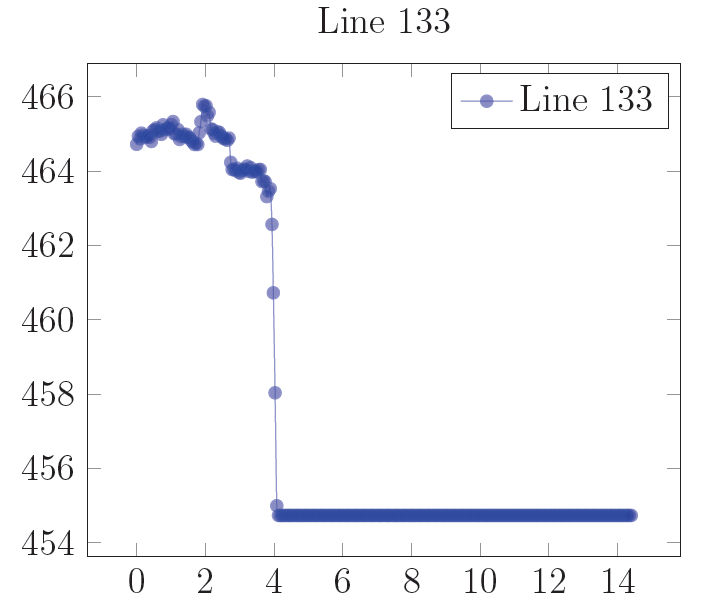
\includegraphics[scale=.35]{exls1}
\end{center}
\end{frame}

\begin{frame}{2 Dimensional Capacity Addition}
\alert{Not convex!}
\begin{center}
\includegraphics[scale=.75]{dfo/fig-heatmap}
\end{center}
\end{frame}

\begin{frame}{Compass Search}
\alert{Stuck in local minima!}
\begin{center}
\includegraphics[scale=.96]{dfo/fig-trialmap}
\end{center}
\end{frame}


\subsection{Auxiliary Information}
\begin{frame}{Line Clustering}

\alert{Outage rates change in clusters!}
\bi
\item Use network information to refine
\ei
\begin{center}
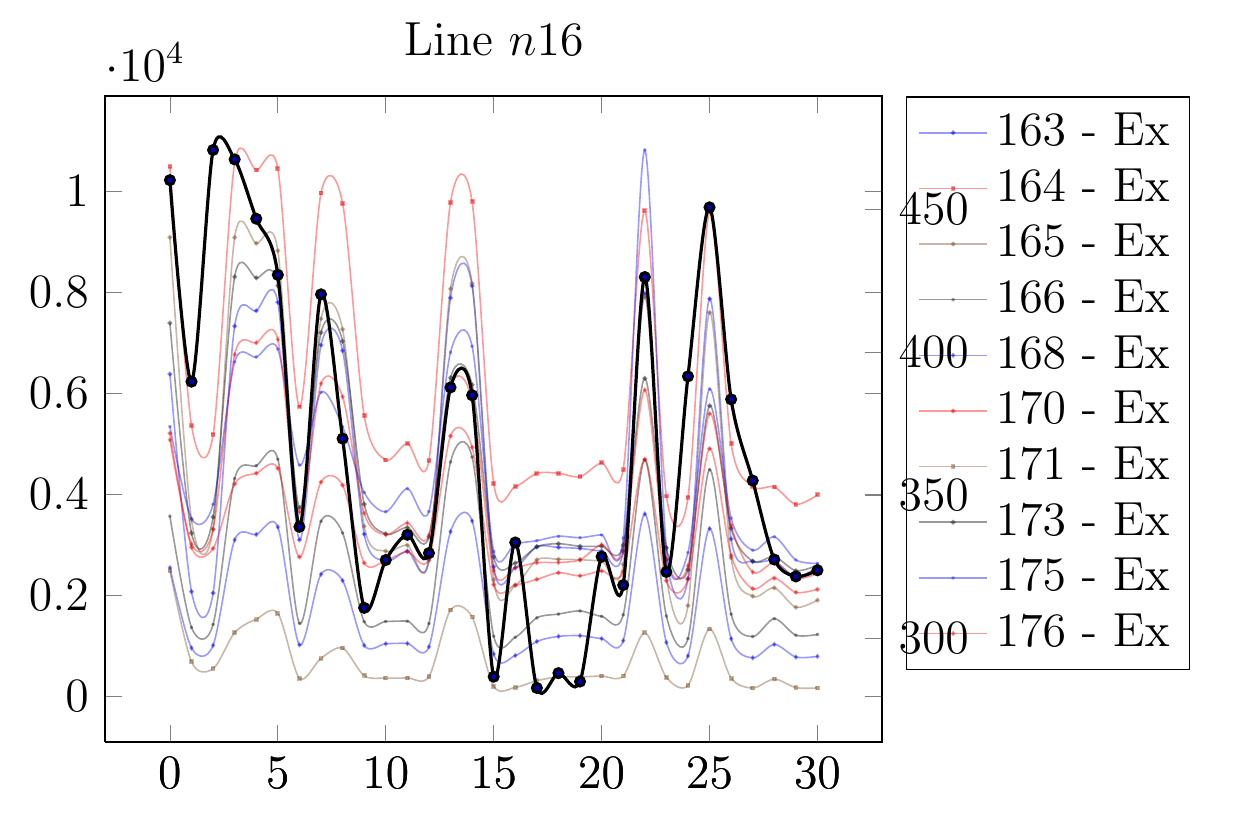
\includegraphics[scale=.3]{clusters}
\end{center}
\end{frame}


\foreach \i in {2, 3, 5,10,25,50}{
\begin{frame}{Breakpoints \i}
\begin{center}
	\begin{tikzpicture}
	\begin{axis}[ scale=.8272, ,legend pos=south east, xlabel={\small Capacity (MW)}, ylabel={\small Load Shed (MW)},xmax=95]	
			\addplot+[opacity=.456775, mark size=.915, only marks,error bars/.cd, y dir=both, y explicit] table[x=cap, y=ex, y error=se] {./data/breakpoint/done.dat};
			\addplot+[red,opacity=.995, mark size=.915, line width=1.25] table[x=cap, y=ls] {./data/breakpoint/nbhd\i.dat};
\addlegendentry{Num. Pts: \i};

	\end{axis}
	\end{tikzpicture}
\end{center}
\end{frame}
}




\subsection{Conclusion}
\begin{frame}{Conclusion}
\bi
\item Modeling cascading power failures
\bi
\item Decision dependent uncertainty and effective capacity
\item Multi-stage stochastic program with mixed-integer variables
\ei
\item Risk model for real-time dispatch
\bi
\item Line loading risk and net injection uncertainty
\item Joint chance constraint and cutting planes to solve
\item Cost risk frontier and sensitivity analysis
\ei
\item Solving design problems
\bi
\item Efficient simulation with common random numbers
\item Enhanced with accessory information from OPA simulation
\ei
\ei
\end{frame}

\end{document}
